%Revisado

A estrutura física consiste em uma cabine retangular fechada, construída em MDF, com dimensões de $40 \times 40 \times 60$ cm (largura, profundidade e altura). O materia, de cor branca e opaca, possui o duplo objetivo de bloquear a luz externa e evitar a contaminação colorimétrica por reflexos das paredes. O equipamento possui um compartimento superior isolado para acomodar as fontes de alimentação e a eletrônica, garantindo que a área inferior de captura fique livre de cabos e sombras indesejadas. O dispositivo de captura foi montado centralizado no teto da estrutura, a uma distância focal aproximada de 40 cm da base onde as amostras são introduzidas (através de uma abertura frontal), garantindo um enquadramento constante. Um esquema técnico detalhado do equipamento é apresentado na Figura \ref{fig:caixa}.

O sistema de iluminação foi projetado estrategicamente para lidar com os desafios ópticos da pluma de algodão. Utilizaram-se duas matrizes de fitas de LED de alta intensidade (2000 lm/m) posicionadas na parte superior, fornecendo luz difusa para minimizar a geração de sombras profundas e brilhos especulares na fibra. O sistema permite a alternância de temperaturas de cor: LEDs de 2800K (luz ``quente'') foram empregados para realçar a reflectância e o amarelamento natural da fibra (+b), enquanto LEDs de 6000K (luz ``fria'', próxima à luz do dia) maximizaram o contraste morfólogico das impurezas superficiais. O protocolo de captura gerou três imagens por amostra: apenas 2800K, apenas 6000K, e ambas simultaneamente, compondo um \textit{dataset} multiespectral robusto para o treinamento das redes.

O módulo de aquisição baseou-se em um sensor CMOS operando a uma resolução de $1280 \times 720$ \textit{pixels}. Optou-se por esta tecnologia devido à sua alta viabilidade de implantação em esteiras industriais, unindo baixo custo e baixo consumo energético, conforme fundamentado na revisão de literatura. O sensor foi acoplado a uma lente grande-angular com campo de visão de 140°, o que permitiu maximizar a área de amostragem do algodão capturada na base do equipamento sem a necessidade de elevar a altura da caixa. As distorções geométricas inerentes a lentes de grande angulação foram mitigadas pelo posicionamento centralizado da amostra.


\begin{figure}[H]
\centering
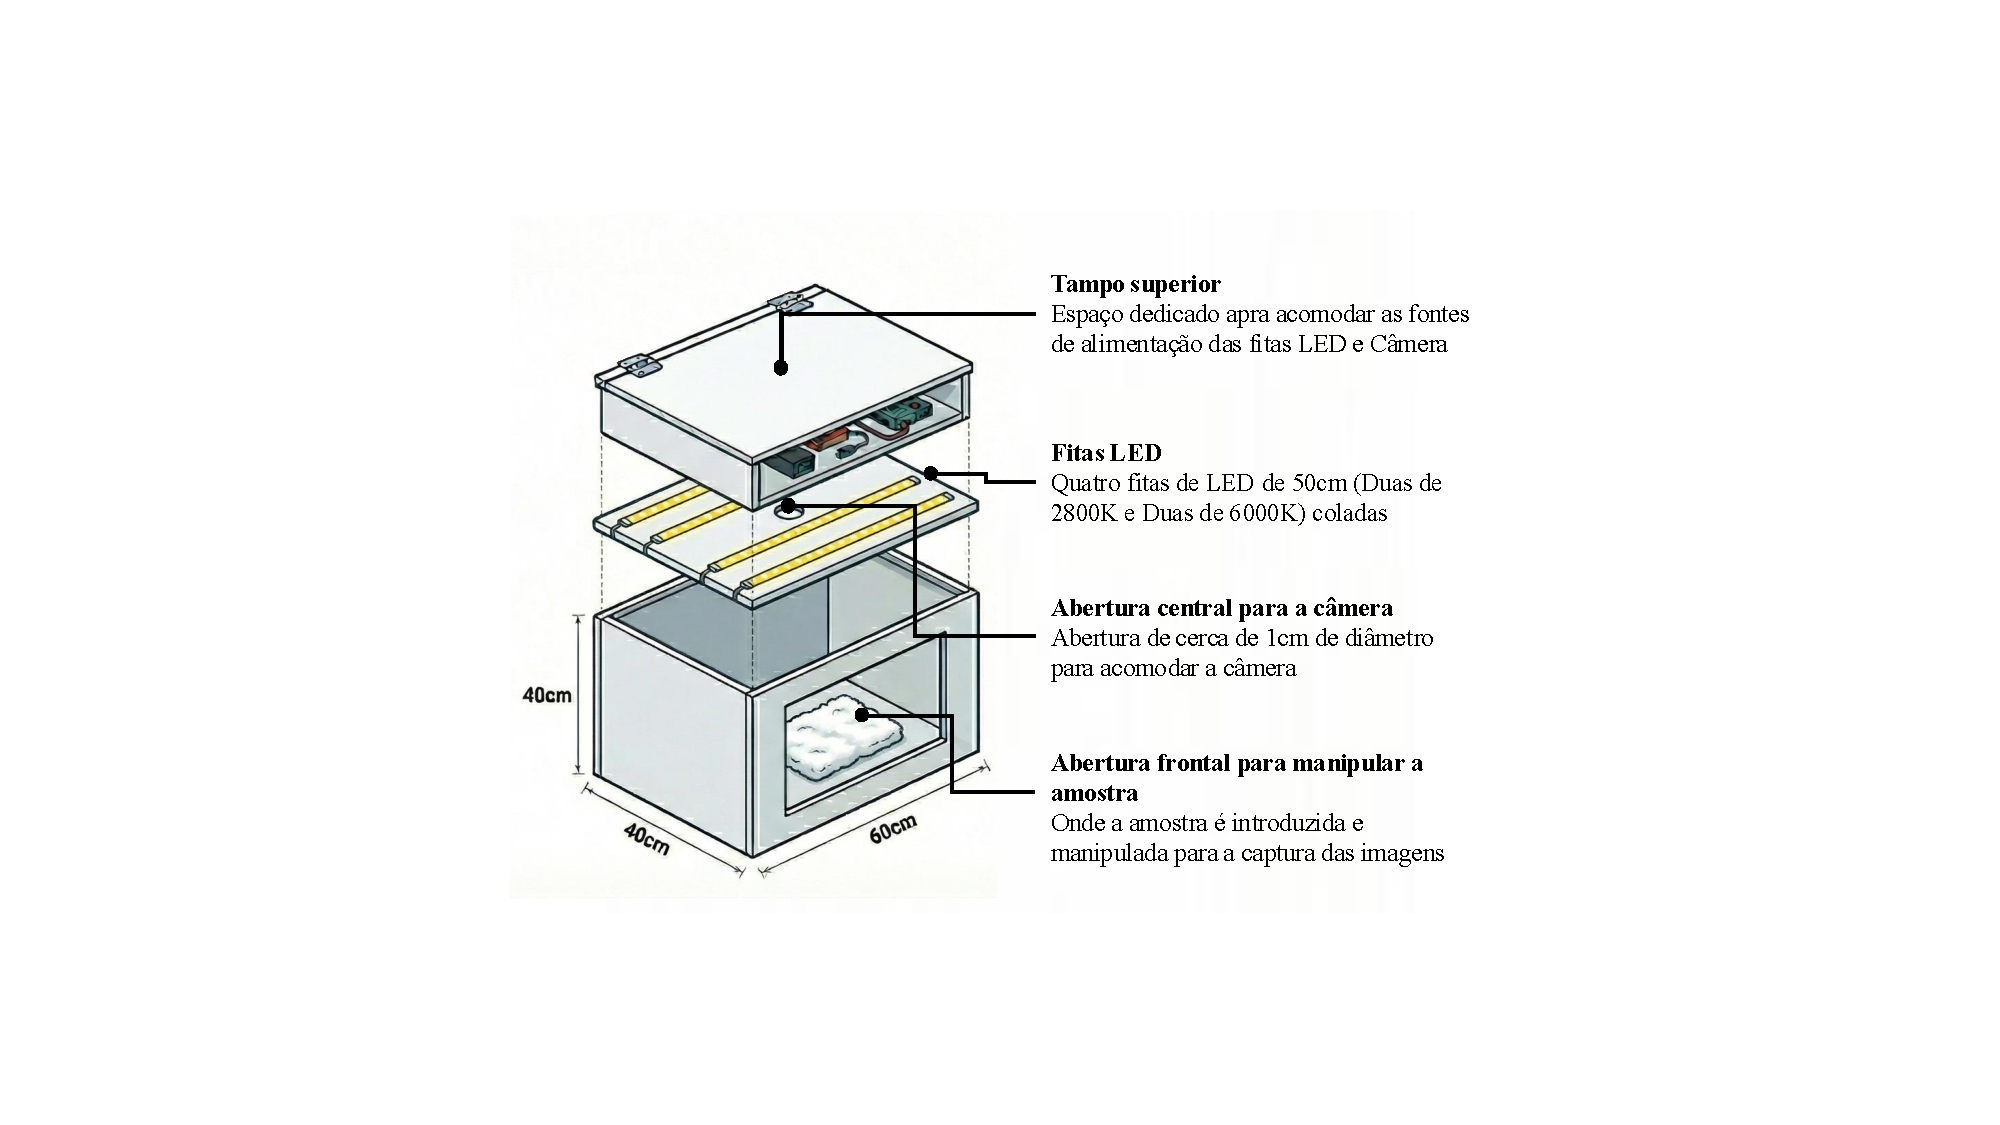
\includegraphics[trim=7.5cm 4cm 7.5cm 4cm, clip, scale=0.9]{images/img_caixa_3.pdf}
% \vspace{-1cm}
\caption{Equipamento de coleta de amostras}
\label{fig:caixa}
\end{figure}